\subsection{Overview}

ActivitySim is an agent-based modeling (ABM) platform for modeling travel demand. Like UrbanSim, the ActivitySim software is entirely open source, and hosted as a part of the Urban Data Science Toolkit\footnote{The open-source Urban Data Science Toolkit is available online at \url{https://github.com/UDST}}. ActivitySim grew in large part out of a need for metropolitan planning organizations (MPOs) to standardize the modeling tools and methods that were common between them in order to facilitate more effective collaboration and sharing of innovations.

Today, ActivitySim is both used and maintained by an active consortium of MPOs, transportation engineers, and other industry practitioners. Because of the cooperative approach taken by ActivitySim stakeholders towards its ownership, and because many of its \enquote{owners} are also its main users, the platform continues to mature in the direction that most benefits the practitioners themselves. ActivitySim development is still in beta, with an official 1.0 release scheduled for 2018.

\subsection{Inputs}

ActivitySim requires two main sets of input data, one relating to geography and the other relating to the population of synthetic agents whose travel choices are being modeled.

The geographic data are stored at the level of the traffic analysis zone (TAZ) and are comprised of three components: 1) land use characteristics; 2) a matrix of zone-to-zone travel impedances (travel times, distances, or costs) specific to the mode of travel and time of day; and 3) a table of user-defined measures of aggregate utility estimated for each zone. In transportation planning, these zone-level impedances and utility measures are commonly referred to as \emph{skims} and \emph{accessibilities}, respectively.

The land use data consist of zone-level population and employment characteristics, along with measures of different land use and building types. In our integrated model these data are read directly from the outputs generated by UrbanSim, but for a single simulation iteration any source of aggregate land use data would suffice.

Travel skims are typically generated by a traffic assignment model, which ActivitySim is not. ActivitySim instead expects to load the skims from an OpenMatrix (OMX) formatted data file\footnote{The OpenMatrix format is specified online at \url{https://github.com/osPlanning/omx/wiki}}. The creation of these skims is described below in Section \ref{sec:ta} on traffic assignment.

Accessibilities can be generated directly from the skims or any other graph representation of the transportation network. They are computed by aggregating mode-specific measures of access to specific amenity types across the network, most commonly employment centers, retail outlets, and transportation hubs. The measures of access can be as simple as counts of amenities reachable within a given shortest-path distance or travel time, or as complex as composite utilities generated by a discrete choice model. 

The second set of ActivitySim input data is the synthetic population. The synthetic population data consist of both individuals and their characteristics, as well as the households and household characteristics into which the individuals are organized. The synthetic population is shared between UrbanSim and ActivitySim, although UrbanSim does not make use of individual-level characteristics.

The exhaustive details of the ActivitySim data schema are documented online\footnote{The ActivitySim data schema is available online at \url{https://udst.github.io/activitysim/dataschema.html}}.

\subsection{How it works}

ActivitySim, like UrbanSim, relies heavily on discrete choice models and random utility maximization theory \citep{mcfadden-1974}. Please refer to Section \ref{sec:urbansim} for specific details about how discrete choice models work within an agent-based microsimulation framework.

An ActivitySim run consists of a series of sequentially executed model steps. The individual models can be grouped into the four clusters---long term decisions, coordinated daily activity patterns, tour-level decisions, and trip-level decisions---illustrated in Figure \ref{fig:asim-models} and summarized briefly here:

\begin{itemize}
    \item \emph{Long-term choice models}: ActivitySim's three long-term choice models---workplace location choice, school location choice, and auto-ownership---model the choices that are not made every day in the real world but have a substantial impact on those that are. These models will eventually be migrated to run directly in the UrbanSim environment so that the time horizons of the two simulation platforms are internally consistent.
    
    \item \emph{Coordinated Daily Activity Patterns}: the CDAP step models the group decision-making process for individual household members all seeking to maximize the utility of their daily activities together. CDAP takes into consideration mandatory and non-mandatory trips choosing activities to maximize each individual's utilities. The maximization process currently involves the estimation of all possible combinations of all individuals within a household, and thus has the longest run-time of all ActivitySim models.
    
    \item \emph{Tour-level decisions}: tours define chains of trips that are completed together without returning home in between. Mandatory tours include trips to and from work and school, while non-mandatory trips are entirely discretionary. Non-mandatory tour alternatives are specified in a user-defined configuration file, and thus these steps include a destination choice model as well. Mandatory tour alternatives have already been computed by the long-term decision models. Each tour type has separate model steps for estimating mode choice, departure time, and the frequency of the tour.
    
    \item \emph{Trip-level decisions}: mode choice must be selected at the level of the individual trip as well as the tour because a given tour may include different modes for different trip legs. Trip departure and arrival times are estimated as well. The rest of the trip characteristics are inherited from the tours to which a trip belongs. 
\end{itemize}

\begin{figure}[htbp]
    \center
    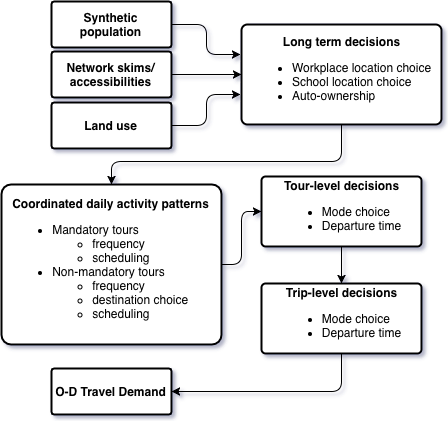
\includegraphics[width=\textwidth]{graphics/asim_flow.png}
    \caption[ActivitySim model flow]{ActivitySim model flow\footnote{The ActivitySim model flow is adapted from \url{http://analytics.mtc.ca.gov/foswiki/bin/view/Main/ModelSchematic}}}
    \label{fig:asim-models}
\end{figure}

\subsection{Outputs}

The output of an ActivitySim run consists of a single HDF5 data file with a single table of results corresponding to each model step, along with the versions of the input files in their final, updated states. For the purpose of generating travel demand for traffic assignment, however, we are only concerned with the output of the trip generation step. This single file contains the origin and destination zones, start and end times, and mode choice for every trip taken by every agent over the course of a day. We then take the subset of these trips that are completed by automobile and aggregate the counts by origin-destination pair and hour of departure. These hourly, zone-level demand files are finally handed off for use in traffic assignment.

\subsection{Calibration and validation}
Compared to their meso- and macro-scale counterparts, microsimulations like ActivitySim more accurately capture the nonlinearities that define most patterns of human behavior by modeling the decision-making processes of individual agents. The models themselves, however, are not meant to be interpreted on the same disaggregate scale. We do not know which individuals will use which mode to complete which activity on a given day, but rather how an entire population of individuals is likely to behave \textit{en masse}.

As such, there are a variety of data sets available to us for validating our results, including the Bay Area Travel Survey (BATS), the U.S. Census Longitudinal Employer-Household Dynamics program (LEHD), and the California Household Travel Survey (CHTS). All of these products offer data that can be aggregated to the TAZ level and compared to the output of our models.